% !TEX root = ../main.tex

\chapter{Background}
\label{chapter:Background}
In this thesis machine learning will be defined as the guided search for candidate functions $f^*: X \to Y$ defined on a data distribution $\mathcal{D}$ to maximize the expectation of an objective function 
${g: X \times Y \to \mathbb{R}}$ using a signal function $g^*$, which is available during train time on the train data distribution $\mathcal{D}_{\text{train}}$:
\begin{equation}
    \label{general_learning_paradigm}
    \begin{aligned}
        f^* &= \arg\max_{f} \mathbb{E}_{x \sim \mathcal{D}}[g(x,f(x))] \\
        f^* &\approx f' = \arg\max_{f} \mathbb{E}_{x \sim \mathcal{D}_{\text{train}}}[g^*(x,f(x))]
    \end{aligned}
\end{equation}

Commonly, $g^*$ is either a (negative) loss or a (positive) reward.

Following the book "Pattern Recognition and Machine Learning" \cite{bishop} there are three learning paradigms common in machine learning: 
\begin{itemize}
	\item Supervised Learning
	\item Unsupervised Learning
	\item Reinforcement Learning.
\end{itemize}

In the following sections, we will provide an overview of these learning paradigms. 
Then, we will introduce the mathematical framework of \ac{mdp}s to model the environment in \ac{rl}. 
After that, we will discuss model-free and model-based algorithms for \ac{mdp}s. We will also introduce \ac{il} and \ac{irl}. 
Next, we will introduce \ac{pomdp}, followed by an overview of sequential models that can be used 
to solve \ac{pomdp}s.

\section{Supervised Learning}
\label{section:super_learn}
Supervised learning is a learning paradigm where the input-output pairs $(x,y) \in X \times Y$ are given, and the goal is to learn a function 
$f^*$ that maps inputs $x \in X$ to outputs $y \in Y$. The objective function is typically a loss function that measures the difference between 
the predicted output $f(x)$ and the true output $y$.

Formally the signal or loss function $L = g^*$ is defined on a training set $\mathcal{D}_{\text{train}} = {(x_i,y_i)}_{i=1}^N$ where $x_i \in X$, $y_i \in Y$ and $N$ is the 
cardinality of the training set. Using the 
labels, it computes a loss between the output of a function $f(x_i)$ and a desired output $y_i$. The signal function is shaped such that optimizing $f$ for $L$ 
over $\mathcal{D}_{\text{train}}$ should be aligned with optimizing $f$ for $g$ over $D$:

\begin{equation}
\begin{aligned}
f^* &= \arg\min_{f} \mathbb{E}_{(x,y) \sim D}[g(f(x), y)] \\
f^* &\approx f' = \arg\min_{f} \mathbb{E}_{(x,y) \sim \mathcal{D}_{\text{train}}}[L(f(x),y)] = \arg\min_{f} \frac{1}{n}\sum_{i=1}^n L(f(x_i),y_i)
\end{aligned}
\end{equation}


Supervised learning can be used for a variety of tasks, including classification, regression, and sequence prediction. In classification, 
the goal is to predict a discrete class label $y \in {1,2,\ldots,K}$ for a given input $x$. In regression, the goal is to predict a continuous 
output $y \in \mathbb{R}$ for a given input $x$. In sequence prediction, the goal is to predict a sequence of outputs $y_1,\ldots,y_T$ for a 
given input sequence $x_1,\ldots,x_T$, as stated in \cite[chapter~4]{bishop} \cite[chapter~5, chapter~6]{Goodfellow}.

\section{Unsupervised Learning}
\label{section:unsup_learn}
Unsupervised learning is a learning paradigm where the input data is unlabeled and the goal is to discover underlying patterns or structure in the data.
The objective function in unsupervised learning is typically not based on a predefined notion of correctness, but
rather on measures of statistical
independence or data compression.

Unsupervised learning can be used for a variety of tasks, including clustering, density estimation, dimensionality 
reduction, and anomaly detection.
It is also often used as a pre-processing step in supervised learning, where the goal is to learn a more informative 
representation of the input data 
for the downstream task \cite[chapter~9]{bishop} \cite[chapter~5]{Goodfellow}. 

\section{Reinforcement Learning}
\label{section:rl}

 \ac{rl} is a learning paradigm where an agent interacts with an environment and learns to take actions that maximize a 
cumulative reward signal. In this paradigm, the input $x$ is typically the state $s$ of the environment, the output $y$ is the action $a$ taken by the agent, 
and the objective function $g$ is a reward signal $r$.

The agent learns a policy $\pi: S \to A$ that maps states to actions, in order to maximize the expected cumulative reward:

\begin{equation*}
    \label{rl_objective}
    \pi^* = \arg\max_{\pi} \mathbb{E}_{\tau \sim p(\tau | \pi)} \left[ \sum_{t=0}^T \gamma^t r_t \right]   
\end{equation*}
\begin{equation}
    \approx \pi' = \arg\max_{\pi} \frac{1}{N} \sum_{i=1}^N \left[ \sum_{t=0}^{T_i} \gamma^t r_{i,t} \right]
\end{equation}

where $\tau = (s_0, a_0, r_0, s_1, a_1, r_1, \ldots, s_T, a_T, r_T)$ is a trajectory, $p(\tau | \pi)$ is the probability of a trajectory 
under policy $\pi$, $\gamma \in [0,1]$ is a discount factor that controls the importance of future rewards, and $N$ is the number of trajectories sampled.

\subsection{Classification of Reinforcement Learning}
%\begin{minipage}{\textwidth}
\begin{itemize}

    \item \textbf{Model type:}
    \begin{itemize}
    \item Model based: The algorithm explicitly models the dynamics of the environment.
    \item Model free: The algorithm learns a policy without explicitly modelling the environment.
    \end{itemize}
    \item \textbf{Action/Observation space:}
    \begin{itemize}
    \item Continuous: The action/observation space is continuous, typically represented by a real-valued vector.
    \item Discrete: The action/observation space is discrete, typically represented by a finite set of actions.
    \end{itemize}
    \item \textbf{Policy type:}
    \begin{itemize}
    \item On-policy: The algorithm learns the optimal policy while using the same policy to collect experience.
    \item Off-policy: The algorithm learns the optimal policy while using a different policy to collect experience.
    \end{itemize}
    \item \textbf{Reward type:}
    \begin{itemize}
    \item Dense reward: The agent receives a reward signal for every time step in the environment.
    \item Sparse reward: The agent receives a reward signal only for certain time steps in the environment.
    \end{itemize}
    \item \textbf{Time horizon:}
    \begin{itemize}
    \item Infinite horizon: The algorithm aims to maximize the expected sum of rewards over an infinite time horizon.
    \item Finite horizon: The algorithm aims to maximize the expected sum of rewards over a fixed time horizon.
    \end{itemize}
    \begin{samepage}
    \item \textbf{inference type:}
    \begin{itemize}
    \item Probabilistic inference: The algorithm samples actions according to a probability distribution.
    \item Deterministic inference: The algorithm chooses an action deterministically.
    \end{itemize}
\end{samepage}
\end{itemize}
%\end{minipage}

\section{Markov Decision Processes}
\ac{mdp}s are a mathematical framework used to model decision-making processes that occur in a sequence. They provide a useful 
context to develop \ac{rl} algorithms.

An \ac{mdp}is defined as a tuple $( S, A, T, R, \gamma )$, where:
\begin{itemize}
    \item $S$ is the set of possible states in the system
    \item $A$ is the set of possible actions that can be taken in each state
    \item $T$ is the transition function that specifies the probability of moving from one state to another given a certain action
    \item $R$ is the reward function that specifies the immediate reward obtained after taking a certain action in a certain state
    \item $\gamma$ is the discount factor that determines the importance of future rewards relative to immediate rewards
\end{itemize}

The transition function $T$ is defined as:

$$T(s, a, s') = \mathbb{P}(s_{t+1}=s' \mid s_t=s, a_t=a),$$
where $s, s' \in S$ and $a \in A$.

This function specifies the probability of moving from state $s$ to state $s'$ after taking action $a$. The reward function $R$ is defined as:

$$R(s, a) = \mathbb{E}[r_{t+1} \mid s_t=s, a_t=a]$$

This function specifies the expected immediate reward obtained after taking action $a$ in state $s$. The discount factor $\gamma$ is a 
parameter that determines the importance of future rewards relative to immediate rewards. It is typically a value between 0 and 1, where 0 means that 
only immediate rewards are important and 1 means that future rewards are equally important. An example diagram is depicted in Figure \ref{fig:mdp_diagram}.

\begin{figure}
    \centering
    \begin{tikzpicture}[scale=0.1]
        % Define nodes
        \node (s1) [circle, draw, fill = green!30] {$s_1$};
        \node (t1_2) [rectangle, draw, right of=s1, xshift=1.5cm] {$T(s_2|s_1, a_1)$};
        \node (s2) [circle, draw, fill = green!30, right of = t1_2, xshift=1.5cm] {$s_2$};
        \node (t2_3) [rectangle, draw, right of=s2, xshift=1.5cm] {$T(s_3|s_2, a_2)$};
        \node (s3) [circle, draw, fill = green!30, right of = t2_3, xshift=1.5cm] {$s_3$};
        \node (r_1) [rectangle, draw, fill = {rgb,255:red,100;green,150;blue,100}, below of=t1_2] {$R(s_1, a_1)$};
        \node (r_2) [rectangle, draw, fill = {rgb,255:red,100;green,150;blue,100}, below of=t2_3] {$R(s_2, a_2)$};

        \node (policy_1) [diamond, draw, fill = yellow!30, above of = s1, yshift=1.5cm] {$\pi$};
        \node (policy_2) [diamond, draw, fill = yellow!30, above of = s2, yshift=1.5cm] {$\pi$};
        \node (policy_3) [diamond, draw, fill = yellow!30, above of = s3, yshift=1.5cm] {$\pi$};

        \draw [->, black!50, line width=2pt] (s1) -- node[midway, above] {} (policy_1);
        \draw [->, black!50, line width=2pt] (s2) -- node[midway, above] {} (policy_2);
        \draw [->, black!50, line width=2pt] (s3) -- node[midway, above] {} (policy_3);

        \draw [->, black!50, line width=2pt] (s1) -- node[midway, above] {} (t1_2);
        \draw [->, black!50, line width=2pt] (s2) -- node[midway, above] {} (t2_3);


        \draw [->, black!50, line width=2pt] (policy_1) -- node[black!100, midway, below] {$a_1$} (t1_2);
        \draw [->, black!50, line width=2pt] (policy_2) -- node[black!100, midway, below] {$a_2$} (t2_3);

        \draw [->, black!50, line width=2pt] (t1_2) -- node[midway, left] {} (s2);
        \draw [->, black!50, line width=2pt] (t2_3) -- node[midway, left] {} (s3);

        \draw [->, color={rgb,255:red,100;green,150;blue,100}, line width=2pt] (t1_2) -- node[midway, left] {} (r_1);
        \draw [->, color={rgb,255:red,100;green,150;blue,100}, line width=2pt] (t2_3) -- node[midway, left] {} (r_2);
    \end{tikzpicture}
  \caption{A \ac{mdp} diagram with an agent that takes in states $s_t$ and outputs action $a_t$.}
  \label{fig:mdp_diagram}
\end{figure}

Importantly, the transition function $T$ satisfies the Markov property. The Markov property characterizes stochastic processes where the future state of the 
process depends only on the current state and not on any past states. Formally a stochastic process has the Markov property if, 
for all time steps $t$, states $s_t$, and actions $a_t$, the following condition holds:

\begin{equation*}
    P(s_{t+1} \mid s_t, a_t, s_{t-1}, a_{t-1}, \ldots, s_1, a_1) = P(s_{t+1} \mid s_t, a_t).
\end{equation*}
In this thesis, we will refer to $r(s_t, a_t)$ as $r_t$, if not indicated otherwise. Moreover, we will use $\tau = \{(a_t, s_t)\}_0^T$ to 
indicate a trajectory with actions $a_t$ and states $s_t$.



\section{Policy Gradient}
The following section follows Sutton \etAl \cite{NIPS1999_464d828b}. There are numerous ways to arrive at a policy that maximizes the \ac{rl} objective as defined in equation 
\ref{rl_objective}. For large or continuous action and observation spaces, a common approach is 
to parametrize the policy using a differentiable function. In this thesis we use neural networks for this task. The expectation over the cumulative 
reward $J$ with respect to a policy $\pi$ with parameters $\theta$ can be written as:

\begin{equation}
J(\theta) = \mathbb{E}_{\tau \sim p(\tau | \pi)} \left[ \sum_{t=0}^T \gamma^t r_t \right]
\end{equation}
where  $p(\tau | \pi)$ is the probability of generating trajectory $\tau$ under policy $\pi$, and $\theta$ are the parameters of the policy $\pi$. 
$T$ can either be finite or infinite. If $T$ is infinite, $\gamma$ must be smaller than 1.

Our goal is to maximize $J(\theta)$ with respect to $\theta$. We can compute the gradient of $J(\theta)$:
\begin{equation}
    \label{nabla_reinforce}
    \begin{aligned}
        \nabla_{\theta} J(\theta) = \mathbb{E}_{\tau \sim p(\tau | \pi)} \left[ \sum_{t=0}^T \nabla_{\theta} \log \pi(a_t|s_t;\theta) \cdot \sum_{t'=t}^T \gamma^{t'-t} r_{t'} \right]\\
        = \mathbb{E}_{\tau \sim p(\tau | \pi)} \left[ \sum_{t=0}^T \nabla_{\theta} \log \pi(a_t|s_t;\theta) \cdot  G_t\right],
    \end{aligned}
\end{equation}
where $G_t = \sum_{t'=t}^T \gamma^{t'} r_{t'}$ and $\pi(a_t|s_t;\theta)$ is the probability of taking action $a_t$ in state $s_t$ under policy $\pi$ with parameters $\theta$. 
$G_t$ represents the total discounted reward obtained after taking action $a_t$ in state $s_t$ and following trajectory $\tau_{i>t}$ after that.

In practice we don't have access to the real expectation. Instead we sample $n$ trajectories and approximate the expectation.
A common choice is to sample one trajectory per update step. 
This finally gives us the gradient of the approximated expected reward with respect to the policy parameters $\theta$. We can use this gradient to update the parameters of the policy in the direction of steepest ascent. Specifically, we can use stochastic gradient ascent to update the policy parameters after observing a trajectory $\tau$:
\begin{equation}
    \label{reinf_update}
    \theta \leftarrow \theta + \alpha \nabla_{\theta} \log \pi(a_t|s_t;\theta) \cdot G_t
\end{equation}
where $\alpha$ is the learning rate. This update rule is used in the REINFORCE algorithm \cite{NIPS1999_464d828b} depicted in algorithm \ref{fig:REINFORCE}.
The algorithm collects 1 trajectory, computes the gradient estimate, and updates the policy parameters using stochastic gradient ascent. 
It continues until convergence.

\begin{algorithm}[H]
    \SetAlgoLined
        \KwIn{Policy function $\pi_{\theta}(a|s)$, learning rate $\alpha$}
        \KwOut{Learned policy parameters $\theta$}
        Initialize policy parameters $\theta$;
        \While{not converged}{
            Sample a trajectory $\tau = (s_1, a_1, r_2, \dots, s_{T-1}, a_{T-1}, r_T, s_T)$ by following the policy $\pi_{\theta}$:\\
            \For{$t\leftarrow 1$ \KwTo $T$}{
                Compute the return starting from time $t$: \\
                $G_t = \sum_{k=t}^T \gamma^{k-t} r_k$ ;\\
                Compute the gradient of the log probability of taking action $a_t$ in state $s_t$: \\
                $\delta_{\pi(\theta)} = \nabla_{\theta}\log \pi_{\theta}(a_t|s_t)$; \\
                Compute the gradient estimate for this time step: \\
                $g_t \leftarrow G_t \delta_{\pi(\theta)}$;
                Update policy parameters using the gradient estimate:
                $\theta \leftarrow \theta + \alpha g_t$;
            }
        }
    \caption{REINFORCE algorithm with one trajectory per update}
    \label{fig:REINFORCE}
\end{algorithm}
    

\section{MDP Model}
Now that we have established the foundation of \ac{rl}, we will investigate two learning paradigms, 
namely model-free \ac{rl} in Section \ref{sec:mod_free_ref} and model-based 
\ac{rl} in Section \ref{sec:mod_based_ref}.

Model-free algorithms aim to learn the dynamics of the system together with the action distribution induced by the policy. In this sense, they learn to predict the posterior 
estimate of the expected rewards given the \ac{mdp} dynamics and the current policy. It is the preferred paradigm in continuous action spaces, 
as it is robust to uncertainties of the \ac{mdp} dynamics and does not need a model of the environment, which is hard to provide in many cases. 
Model-based approaches learn the policy given a model of the MDP. If the model is not known, it is learned 
from observed interactions. The advantage of model-based algorithms is, that the policy can use the model to plan steps ahead. 
Where it is applicable, planning has proven to be 
a crucial advantage. One example is the MuZero algorithm from Julian Schrittwieser et. al \cite{MUZero}.

\section{Model-Free Learning}
\label{sec:mod_free_ref}
In the following section we develop the framework of value functions, on which off-policy algorithms rely. 
We will then introduce \ac{ppo}, a state-of-the-art on-policy algorithm and \ac{tqc}, a state-of-the-art off-policy algorithm, 
which we will use as part of our baselines.

\subsection{Value Functions}

The following section follows Sutton and Barto \cite{sutton2015reinforcement}. Value functions are a fundamental concept in \ac{rl} and are used to estimate the expected return of being in a 
particular state or taking a particular action. In this section we discuss the two main types of value functions in \ac{mdp}s: state 
value functions and state action value functions.

\subsubsection{State Value Function}

The state value function $V_{\pi}(s)$ is the expected return when starting in state $s$ and following policy $\pi$ thereafter. It is defined as:

\begin{equation}
    \label{eq:value_func_proper}
    V_{\pi}(s) = \mathbb{E}_{\tau \propto \pi}\left[\sum_{t=0}^{\infty} \gamma^t r_t \mid s_0 = s\right].
\end{equation}

$\mathbb{E}_{\tau \propto \pi}$ denotes the expected value under policy $\pi$.

The state value function satisfies the Bellman equation, which expresses the relationship between the value of a state and the values of its successor states:

\begin{equation}
    \label{bootstrap_v}
    \begin{aligned}
        V_{\pi}(s) = \mathbb{E}_{\tau \propto \pi}\left[\sum_{t=0}^{\infty} \gamma^t r_t \mid s_0 = s\right] \\
        = \sum_{a \in \mathcal{A}} \pi(a \mid s) \left[ r(a,s)  + \gamma \sum_{s' \in \mathcal{S}} p(s' \mid s,a) \sum_{a' \in \mathcal{A}} \pi(a' \mid s') \left[ r(a',s') + \gamma ...\right] \right]\\
        = \sum_{a \in \mathcal{A}} \pi(a \mid s) \left[ r(a,s) +  \gamma \sum_{s' \in \mathcal{S}} p(s' \mid s,a) V_{\pi}(s')\right]
    \end{aligned}
\end{equation}

where $\mathcal{A}$ is the set of possible actions, $\mathcal{S}$ is the set of possible states, $p(s' \mid s,a)$ is the transition probability 
from state $s$ to state $s'$ under action $a$, $r(s,a)$ is the reward received in state $s$ with action $a$, and $\gamma \in [0,1]$ is the discount factor. 
This formulation assumes a discrete action space,
however it can be adapted for continuous cases by changing the summation with an integral over the probability density function.

\subsubsection{State Action Value Function}

The state action value function, also known as the Q-function, is the expected return when starting in state $s$, taking action $a$, and then following 
policy $\pi$. It is defined as:

\begin{equation}
    Q_{\pi}(s, a) = \mathbb{E}_{\tau \propto \pi}\left[\sum_{t=0}^T \gamma^t r_t \mid s_0 = s, a_0=a\right].
\end{equation}

The state action value function also satisfies the Bellman equation:

\begin{equation}
    \label{bmeq_q}
    Q_{\pi}(s,a) = r(s,a) + \sum_{s' \in \mathcal{S}} p(s' \mid s,a) \left(\gamma \sum_{a' \in \mathcal{A}} \pi(a' \mid s') Q_{\pi}(s',a')\right).
\end{equation}

Both value functions can be expressed in terms of the respective other value function using the Bellman equation:
\begin{equation}
    \label{q_from_v}
    Q_{\pi}(s,a) = r(s,a) + \gamma \mathbb{E}_{s'\propto T(s,a,s')}\left[ V_{\pi}(s') \right]
\end{equation}

and 

\begin{equation}
    V_{\pi}(s) = \mathbb{E}_{a \propto \pi(\cdot|s)} \left[ Q_\pi(s,a) \right]
\end{equation}



\subsection{Temporal Difference Learning}
\label{subsection:TD_learning}
Temporal Difference (TD) learning is a paradigm that learns the value function from experience by updating its value based on the difference between the predicted reward and the actual reward received at each time step.

The update rule for TD learning is derived from the Bellman equation as stated in \ref{bootstrap_v}.

The idea behind TD learning is to update the value function V(s) iteratively based on the difference between the predicted reward and the actual reward received at each time step t. This difference is known as the temporal difference error $\delta$:
\begin{equation}
    \label{TD_update}
    \delta_t = r_t + \gamma V(s_{t+1}) - V(s_t).
\end{equation}
The update rule for the value function in TD learning is:
$$V(s_t) \leftarrow V(s_t) + \alpha \delta_t$$

where $\alpha (0 < \alpha \leq 1)$ is the learning rate, which determines the weight given to new information relative to old information. TD learning for the $Q$ 
value is analogous. Recursively plugging in the temporal difference error n times is referred to as n-step TD learning. For example, 2-step TD learning can be written as 
$\delta_t = r_t + \gamma (r_{t+1} + \gamma V(s_{t+2}) - V(s_{t+1})  ) - V(s_t)$.

Iterating the value function estimate according to the update rule \ref{TD_update} is guaranteed to converge to the real value function of $\pi$. To see this, 
let $V$ be the value function estimate and $V_{\pi}$ be the true value function for policy $\pi$ as defined in equation \ref{bootstrap_v}. Also let $T$ be the 
Bellman update operator defined as:

\begin{equation}
    (T V)(s) = E_{\tau \propto \pi} \left(r(s,a) + \gamma \sum_{s' \in S} p(s' \mid s,a) V(s')\right).
\end{equation}
It follows from this equation, that the expectation of the TD error defined in Equation \ref{TD_update} can be expressed from the Bellman operator $T$ as 
\begin{equation}
    \label{TD_update_BM}
    \delta_t = (T V)(s_t) - V(s_t),
\end{equation} 
so 
\begin{equation*}
    V^{t+1} = V^t + \delta_t = (T V)^t
\end{equation*}
We want to proof that $V$ converges to $V_{\pi}$ under the action of the update operator $T$. We will do this in two steps:
\begin{enumerate}
    \item show that $T$ is a contraction mapping,
    \item show that the unique fixed point of $T$ given policy $\pi$ is the true value function $V_{\pi}$.
\end{enumerate}

\textbf{Step 1:} Contraction property\\
\textbf{Definition:}\\
Let $(X, d)$ be a complete metric space. A map $\mathcal{B}:X \rightarrow X$ is called a contractor if there exists a factor $\gamma \in [0, 1)$ s.t.
\begin{equation}
    d(\mathcal{B}(x), \mathcal{B}(y)) \leq \gamma d(x,y) \quad \forall x,y \in X.
\end{equation}
\\ 

\textbf{Banach Fixed Point Theorem:}\\
Let (X,d) be a complete metric space and $\mathcal{B}:X \rightarrow X$ a contractor. 
Then $\mathcal{B}$ has a unique fixed point $x^* \in X$, s.t. $\mathcal{B}(x^*) = x^*$, as discussed by Agarwal \etAl \cite{agarwa}. The sequence $\text{lim}_{n \rightarrow \infty}\mathcal{B}^n(x)$ converges to $x^*$.

First we will show that $T$ is a contraction mapping with respect to the infinity norm. Let $V$ and $W$ be two value function estimates. Then we have:

\begin{equation}
    |(TV)(s) - (TW)(s)|_\infty =  
\end{equation}
\begin{equation*}
    \max_{s \in S}\left|E_{\tau \propto \pi}\left(r(s,a) + \gamma \sum_{s' \in S} p(s' \mid s,a) V(s')\right) -E_{\tau \propto \pi}\left(r(s,a) + \gamma \sum_{s' \in S} p(s' \mid s,a) W(s')\right)\right| 
\end{equation*}
\begin{equation*}
    = \max_{s \in S}\gamma \sum_{s' \in S} p(s' \mid s,a) |V(s') - W(s')| 
\end{equation*}
\begin{equation*}
    \leq \max_{s \in S}\gamma \sum_{s' \in S} p(s' \mid s,a) \max_{s'' \in S}|V(s'') - W(s'')| 
\end{equation*}
\begin{equation*}
    = \gamma |V - W|_\infty
\end{equation*}

where the last equality comes from the fact that probability distributions are normalized: $\sum_{s' \in S} p(s' \mid s,a) = 1$ and 
$|V(s'') - W(s'')|$ is independent of $s'$.

Therefore, $T'$ is a contraction mapping with respect to the infinity norm. \\

\textbf{Step 2:} Unique fixed point\\
By the Banach fixed point theorem, $T$ has a fixed point $TV^* = V^*$. 
We see, that this fixed point satisfies the Bellman Equation \ref{bootstrap_v} with 
$$TV^* = E_{\tau \propto \pi} \left(r(s,a) + \gamma \sum_{s' \in S} p(s' \mid s,a) V^*(s')\right).$$
As the fixed point is unique, this proves that iteratively applying $TV$ will converge to $V_{\pi}$. Following \ref{TD_update_BM} it is shown that for small enough 
update rates $\alpha$, TD learning converges to the true value function. A similar proof can be found for TD learning of the $Q$ value function.


\subsection{Actor Critic Algorithm}
\label{AC-Alg}
One problem with REINFORCE is, that $G_t$ is computed from the rollout of a whole trajectory. As the policy changes with respect to the update step, this update 
rule can only be used once on a sampled trajectory, making it sample inefficient. An idea is to approximate the expectation over $G_t$ using another neural network, so that an update can be made after every step, 
rather then after the whole trajectory. This approximation is referred to as a "critic" in the actor critic method.

\subsubsection{Critic}
In this section, we will derive an expression to approximate $G_t$ by using an iterative update step with guaranteed convergence.
Revisiting Equation \ref{nabla_reinforce} we define: 
\begin{equation}
    \label{ac policy update}
    \begin{aligned}
        \nabla_{\theta} J(\phi) = \mathbb{E}_{\tau \sim p(\tau | \pi_{\phi})} \left[ \sum_{t=0}^T \nabla_{\phi} \log \pi(a_t|s_t;\phi) \cdot  G_t\right]\\
        = \mathbb{E}_{s_0, a_0, ... ,s_T, a_T \propto \pi} \left[
            \sum_{t=0}^{T}\nabla_{\phi} log \pi_{\phi}(a_t|s_t) \mathbb{E}_{r_t...r_T \propto \pi} \left[ G_t \right]
        \right],
    \end{aligned}
\end{equation}
where 

\begin{align}
    \mathbb{E}_{s_t, a_t, r_t...s_T, a_T, r_T \propto \pi} \left[ G_t \right] \\
    = r(s_t,a_t) + \gamma \mathbb{E}_{s_{t+1} \propto T(s_{t+1}|s_t, a_t)}\left[\mathbb{E}_{a_{t+1} \propto \pi(\cdot|s_t)}  \left[Q_{\pi}(s_{t+1},a_{t+1})\right]  \right]
    = Q_{\pi}(s_{t},a_{t}).
\end{align}


Plugging in the definition of the $Q$-value recursively gives us the Bellman equation for $Q$-values:
\begin{equation*}
Q_{\pi}(s_t, a_t) 
\end{equation*}
\begin{equation*}
    = \mathbb{E}_{\tau \propto p(\tau|\pi)} \left[ r(s_t,a_t) + \gamma Q_{\pi}(s_{t+1}, a_{t+1})\right]
\end{equation*}
for the sequence $\tau = (s_0,a_0, s_1, a_1...) \propto \pi$.

One way to approximate the $Q$ value using a neural network with parameters $\theta$ is to use the temporal difference term as defined in \ref{TD_update_BM} for the $Q$ value:
\begin{equation}
    \label{Q-ValueTD}
    \delta_t = (T Q_{\theta})(s_t) - Q_{\theta}(s_t) = r_t + \gamma Q_{\theta}(s_{t+1}, a_{t+1}) - Q_{\theta}(s_{t}, a_{t}).
\end{equation}
Using the mean squared $J$ of $\delta_t$ as a loss function we get the update:
\begin{equation}
    \nabla_{\theta} J(\theta) = \nabla_{\theta} \mathbb{E}_{\tau \propto \pi}((T Q_{\theta})(s_t, a_t) - Q_{\theta}(s_t, a_t))^2.
\end{equation}
We can use this to update the $Q$ function using the learning rate $\alpha$ with $\theta_{i+1} = \theta_i + \alpha \nabla_{\theta} J(\theta)$. As shown for the value 
function, this update rule is guaranteed to converge to $Q_{\pi}$ with sufficiently small $\alpha$.

\subsubsection{Actor}
Once we have an estimate of the state value function, we can use policy gradient to update our policy $\pi_{\phi}$ with parameters $\phi$:
\begin{equation}
    \label{AC_general_update}
    \nabla_{\phi} J(\phi) = \mathbb{E}_{\tau \sim p(\tau | \pi_{\phi})} \left[\nabla_{\phi} \log \pi(a_t|s_t;\phi) Q_{\theta}(a_t, s_t) \right]
\end{equation}

This defines two update steps, one for the policy and one for the critic. Commonly this approach is called deep deterministic policy gradient or DDPG \cite{lillicrap2019continuous}. 
Some algorithms don't use the $Q$ value for the update step of the policy, but a closely 
related value, called the advantage $A_t$ defined as $A_t = -V(s_t) + r_t + \gamma r_{t+1} + \cdots + \gamma^{T-t+1} r_{T-1} + \gamma^{T-t} V(s_T)$ \cite{A2C}. For the one step 
unroll of the rewards, this value becomes $A_t = Q(a_t, s_t) - V(s_t)$. 
Intuitively, the advantage $A$ is a measure for how good a specific action $a$ is compared to the average action taken by the current policy. 
A proof for the convergence and optimality of this estimator can be found in \cite{proof_A}.

\subsection{Soft Actor Critic}
\label{SAC}
Tuomas Haarnoja \etAl \cite{haarnoja2018soft} developed a new approach for exploration called "Soft Actor-Critic" (SAC). Exploration vs. exploitation 
is a fundamental trade-off in \ac{rl}. An agent must exploit the current knowledge to maximize the cumulative reward it receives 
over the course of its interactions with the environment. Also, the agent must explore new actions and states to improve its knowledge and avoid getting stuck in suboptimal policies. 
The balance between exploration and exploitation is crucial for the success of \ac{rl} algorithms, and different methods aim to find a good compromise between them.

SAC extends the AC method by introducing a new objective that encourages the policy to be more stochastic. Specifically, the SAC algorithm maximizes a modified 
version of the expected cumulative reward that takes into account both the expected reward and the entropy of the policy. The modified objective is given by:

\begin{equation}
J(\pi) = \mathbb{E}_{s_t \sim \mathcal{D}, a_t \sim \pi}[r(s_t, a_t) + \alpha \mathcal{H}(\pi(\cdot|s_t))]
\end{equation}

where $\mathcal{D}$ is the replay buffer, $r(s_t, a_t)$ is the immediate reward for taking action $a_t$ in state $s_t$, and $\mathcal{H}(\pi(\cdot|s_t))$ is the entropy of the policy. The entropy 
encourages the policy to explore different actions, while the temperature parameter $\alpha$ controls the trade-off between exploration and exploitation. In the original implementation, 
SAC uses two $Q$ value estimates and a state value estimate $V$. $V$ is learned given by:

\begin{equation}
    V_{\psi}(s_t) = \mathbb{E}_{a_t \sim \pi_{\phi(a_t|s_t)}}[q_\text{min}(s_t, a_t) - \alpha \log \pi_{\phi(a_t|s_t)}],
\end{equation}
with the minimum value of the two $Q$ critics $Q_\text{min}$ to compensate for the overestimation bias of critics in actor critic 
algorithms. A formal derivation of this bias is done by Thrun and Schwartz \cite{thrun1993issues}. 
The $Q$ values are trained with TD learning:

\begin{equation}
    \mathcal{J}(Q_{\theta_i}) = \mathbb{E}_{(s_t, a_t, r_t, s{t+1}) \sim \mathcal{D}}[(q_{\theta_i}(s_t,a_t) - y_t)^2]
\end{equation}

where $y_t = r(s_t, a_t) + \gamma \mathbb{E}_{s_{t+1} \sim p}[V(s_{t+1})]$ is the target value. This is the same update rule as derived in Equation \ref{Q-ValueTD}, 
considering the identity \ref{q_from_v}.

The policy is updated to minimize the Kullback-Leibler (KL) divergence to the normalized $Q$-Values:
\begin{equation}
    \label{sac_pol_obj}
    J_\pi(\phi_{i}) = D_{\mathrm{KL}} \left( \pi_{\phi_{i}}(\cdot|s_t) || \frac{\exp(Q_{min, {\theta_i}}(\cdot|s_t))}{\underset{a}{\sum}  \exp(Q_{\theta_i}(a|s_t))} \right).
\end{equation}

The KL divergence is a measure of the alikeness of two distributions $P(x)$ and $Q(x)$ over the same sample space $X$:
\begin{equation}
    \label{KL}
    \mathrm{KL}(P\|Q) = \int_{x\in X} P(x) \log \frac{P(x)}{Q(x)} \mathrm{d}x
\end{equation}
It is non-negative, asymmetric in the distributions and $\mathrm{KL}(P\|Q) = 0$ if and only if $P = Q$. In addition to that, it can be differentiated, making it 
a common choice in deep learning applications.

This approach also leads to provably optimal policies, as shown in the appendix B3.1 of the SAC paper \cite{haarnoja2018soft}. 
The policy is inherently stochastic and returns an action according to a spherical gaussian distribution with noise vector $\epsilon_t$, learned mean and variance $a_t = f_{\phi}(\epsilon_t;s_t)$. 
To approximate the derivative of \ref{sac_pol_obj} given limited sample size, the reparameterization trick is used:
   
\begin{align}
 \label{SAC_update_rule}
    \nabla_{\phi}J_\pi(\phi_{i}) \approx \mathbb{E}_{\mathcal{D}} [\nabla_{\phi} log (\pi(\phi_{i})(a_t, s_t))\\
    + \left( \nabla_{a_t} log (\pi(\phi_{i})(a_t, s_t)) - \nabla_{a_t} Q_{\theta_i}(a_t, s_t) \right) \nabla_{\phi} f_{\phi}(\epsilon_t;s_t)].
\end{align}

To summarize, SAC introduces a parameter $\alpha$ with which the trade-off between exploration and exploitation can be tuned. It outperforms non-stochastic 
policies in a number of challenging tasks including robot manipulation tasks with large, continuous action spaces.

\subsection{Trust Region Policy Optimization}
\label{sec:TRPO}
Trust Region Policy optimization \cite{TRPO} aims to find a policy update step with a provable lower bound on value improvement. 
Recall, we defined the \ac{rl} objective as:
\begin{equation}
    J(\pi) = \mathbb{E}_{s_0, a_0, ...}\left[\sum_{t=0}^{\infty}  \gamma^t r(s_t) \right].
\end{equation}
We can compute $J(\tilde{\pi})$ for a different policy $\tilde{\pi}$ using $J(\pi)$ like:
\begin{equation}
    J(\tilde{\pi}) = J(\pi) + \mathbb{E}_{s_0, a_0, ... \propto \tilde{\pi}}\left[ \sum_{t=0}^{\infty}  \gamma^t A_{\pi}(s_t, a_t)\right],
\end{equation}
with the advantage function $A_{\pi}(s_t, a_t) = Q_{\pi}(s_t,a_t) - V_{\pi}(s_t)$. Note that the expectation of the states and actions is taken with respect to 
$\tilde{\pi}$. 
We now introduce the occupancy measure $\rho_{\pi}:\mathcal{S} \rightarrow \mathbb{R}$ for states, which measures how often a state is visited, given a policy:
\begin{equation*}
    \rho_{\pi} = \mathbb{E}_{\tau \propto \pi} \left[ \sum_{t=0}^\infty \gamma^t P(s_t=s) \right].
\end{equation*}
With this, we can define a local approximation $L$ to $J(\tilde{\pi})$:
\begin{equation}
    L_{\pi}(\tilde{\pi}) = J(\pi) + \sum_{s \in S} \rho_{\pi}(s) \sum_{a \in A} \tilde{\pi}(a|s) A_{\pi}(s,a),
\end{equation}
where we used the occupancy measure and advantage function of $\pi$, but the policy $\tilde{\pi}$. This is a useful quantity for policy update algorithms. 
Let's say we have policy $\pi$ and collect statistics by generating trajectories from it to approximate $J(\pi)$ and $\rho(\pi)$. We now want to change the policy 
such that our expected value $J$ improves $J(\tilde{\pi}) > J(\pi)$, but we don't have an estimate of $J(\tilde{\pi})$ before we use $\tilde{\pi}$. 
However, given the current data from policy $\pi$ we can compute $L_{\pi}(\tilde{\pi})$. It has been shown, that the following lower bound on policy 
improvement holds:
\begin{equation*}
    J(\tilde{\pi}) \geq L_{\pi}(\tilde{\pi}) - C D^{\max}_{\operatorname{KL}} (\pi,\tilde{\pi}),
\end{equation*}
\begin{equation*}
    \text{where}\quad C = \frac{4\epsilon}{\gamma/(1-\gamma)^2}\
\end{equation*}
\begin{equation}
    \label{eq:pol_impr_TRPO}
    \text{and} \quad  D^{\max}_{\operatorname{KL}} (\pi,\tilde{\pi}) = \max_s D_{\operatorname{KL}} (\pi(\cdot|s),\tilde{\pi}(\cdot|s)).
\end{equation}
Following this insight, the authors propose an algorithm that aims to maximize expected policy improvement under a $\operatorname{KL}$ divergence constraint. 
We will not explain their algorithm here, as the \ac{ppo} algorithm builds upon this insight, but is computationally cheaper and has been empirically shown to have 
similar or better performance than \ac{trpo}.

\section{Model-Based Learning}
\label{sec:mod_based_ref}
In model-based \ac{rl} the actor has access to the transition model $\mathcal{T}(s, a, s')$ of the MDP. Given this transition model, it can predict the 
expected reward of a sequence of actions given the current state. With this prediction, the agent can use planning algorithms to find an action sequence 
$a_{1, ..., T}$ to optimize the expected reward $J(a_{1:T}) = \mathbb{E}_{\tau \propto a, s_1}\sum_{t=1}^T \gamma^t r_t$. If the algorithm has to learn the transition model, the 
expectation is built with respect to the current estimate of the transition model $\mathcal{T}'(s,a,s')$ with 
$J(a_{1:T}) = \mathbb{E}_{s_t \propto T'(s_{t-1}, a_t, s_t)}\sum_{t=1}^T \gamma^t r_t.$

As shown by Xu \etAl \cite{NEURIPS2020_b5c01503}, a policy based on a learned 
model of the environment has a quadratic error in $\gamma$. Formally let $V_{\pi}^{M^*}$ be the optimal value function for the environment with model $M^*$ and
and let $V_{\pi}^{M_\theta}$ be the value function, given $\pi$ is the optimal policy for the learned model $M_{\theta}$. It is shown, that 
$|V_{\pi}^{M^*} - V_{\pi}^{M_\theta}| \le c \cdot \frac{1}{(1 - \gamma^2)}$, where $c$ is dependent on the KL divergence between the model $M_{\theta}$ and $M^*$. 
Intuitively, with higher $\gamma$, the value function $V_{\pi}^{M_\theta}$ can further deviate from the optimal value 
function $V_{\pi}^{M^*}$.

Considering these findings, it is obvious that most successful applications of this framework are in cases where the model is known or 
the action space is discrete, to make the task of learning the model easier.

\subsection{Proper Value Equivalence}
\label{sec:prop_val_eq}
So far we have stated, that the proper transition function $T(s,a,s')$ must be known or learned for model-based learning. However this is not strictly the case. Recall, we are 
interested in optimizing the expected reward $J$. When we plan n steps ahead to choose the best sequence of actions, we are not interested in the exact state $s_t$ 
of our environment at each time step, but only in the rewards $r_t$.

This insight has been formalized by Christopher Grimm et. al \cite{grimm2021proper} by defining a proper value equivalence model class of an MDP. For that 
let $\mathcal{T}^m_{\pi}(V)$ be the Bellman update for policy $\pi$ given the actual transition function $m$ of the \ac{mdp} and let 
$\mathcal{T}^{m'}_{\pi}(V)$ be another Bellman update given a model $m'$. A model $m'$ is $k^{th}$ order value equivalent to $m$, 
if $k$ applications of the Bellman operator result in the same updated value function: 
\begin{equation}
    \label{eq_kthVE}
    \left(\mathcal{T}^{m}_{\pi}(V)\right)^k = \left(\mathcal{T}^{m'}_{\pi}(V)\right)^k.
\end{equation}
It can be shown, that for $\lim_{k \rightarrow \infty}$ the value function $V_{\pi}^{m'} = V_{\pi}^m$ for every policy $\pi$. Recall, the value function is 
defined as $V_{\pi}(s) = \mathbb{E}_{\tau \propto \pi}\left[\sum_{t=0}^{\infty} \gamma^t r_t \mid s_0 = s\right]$. A model $m'$ that is proper value 
equivalent to $m$, but does not predict the observations or states is sometimes referred to as a "weakly grounded model".

From this work we conclude that solving the 
\ac{rl} problem on $m'$ is guaranteed to find a policy $\pi$ that is optimal for the actual \ac{mdp} with model $m$. 

\section{Imitation Learning}
Imitation learning (\ac{il}) is a type of supervised learning in which an agent learns a policy by observing expert demonstrations, 
rather than by trial and error \cite{IL}. In this approach, the data distribution seen during test time is dependent on the learned policy, 
breaking the \ac{iid} assumption typically made in supervised learning. This means that the performance of the 
learned policy can be severely impacted by distributional shifts between the training data and the test data.

Formally \ac{il} can be defined as the task of learning a policy $\pi^*$ that maximizes the expected discounted sum over rewards during test time, given a dataset of expert demonstrations $D = {s_1, a_1, ..., s_T, a_T}$:

\begin{equation}
    \pi^* = \underset{\pi}{\text{argmax}}\left[\mathbb{E} [\sum_{t=0}^{\infty} \gamma^t r(s_t, a_t)]\right]
\end{equation}

where $s_t$ is the state at time step $t$, $a_t$ is the action taken by the agent at time step $t$, $r(s_t, a_t)$ is the reward received for taking action $a_t$ in state $s_t$, and $\gamma \in [0,1]$ is the discount factor.

Returning to our general learning paradigm \ref{general_learning_paradigm}, $g^*$ has access to expert Data $D_{\text{expert}}$. 
The challenge of \ac{il} 
opposed to the general supervised learning paradigm is, that the data distribution during test time depends on the learned policy $\pi_{\text{imitation}}$:
\begin{align}
    \mathbb{E}_{\mathcal{D} \propto \pi_{\text{imitaion}}}[\sum_{t=0}^{\infty} \gamma^t r(s_t, a_t)] \neq \mathbb{E}_{\mathcal{D} \propto \pi_{\text{expert}}}[\sum_{t=0}^{\infty} \gamma^t r(s_t, a_t)]
\end{align}
in general.

The goal of \ac{il} is to learn a policy that performs as well as the expert demonstrations in a new, unseen environment. 
This approach has been applied successfully in a variety of domains, including robotics \cite{stepputtis2020languageconditioned}, video games \cite{MUZero}, 
and natural language processing \cite{brown2020language}.

\subsection{Behavioral Cloning}
Behavioral cloning is a popular technique used in \ac{il}. 
In behavioral cloning, the policy is learned by minimizing the difference between the actions taken by the expert and the 
actions predicted by the learned policy. Formally let $a_{\text{expert}}$ be the action taken by the expert and $a_{\text{imitation}}$ be the action 
predicted by the learned policy. The goal is to minimize the expected distance between the two actions:

\begin{equation}
\min_{\theta} \mathbb{E}{(s, a_{\text{expert}}) \sim D_{\text{expert}}} [d(a_{\text{expert}}, a_{\text{imitation}})]
\end{equation}

where $d(\cdot, \cdot)$ is a distance metric, and $\theta$ are the parameters of the learned policy. The distance metric could for example be the mean 
squared error, or the cross-entropy loss.


\subsection{Behavioral Cloning for Stochastic Policies}
Behavioral cloning for stochastic policies is a variant of behavioral cloning that is suited for learning policies that output probability distributions over actions. In this setting, the goal is to maximize the probability of the learned policy selecting the action proposed by the expert, rather than simply minimizing the distance between the expert and learned actions. 
A common choice to achieve this is to minimize the KL divergence between the expert policy and the trained policy.

Formally, let 

\begin{center}
    $\pi_{\text{expert}}(a|s) = 
        \begin{cases}
            1 \ |\ (a|s)\in \mathcal{D}_{\text{expert}}\\
            0, \text{else}
        \end{cases}$
\end{center}

be the probability of the expert selecting action $a$ in state $s$, and let $\pi_{\theta}(a|s)$ be the probability of the learned policy. Then the KL divergence can be approximated by
\begin{equation}
    D_{\mathrm{KL}}(\pi_{\text{expert}} || \pi_{\theta}) \approx \sum_{a,s \in \mathcal{D}_{\text{expert}}} \pi_{\text{expert}}(a,s) \log\left(\frac{\pi_{\text{expert}}(a,s)}{\pi_{\theta}(a|s)}\right)
\end{equation}

Differentiating the KL divergence with respect to $\theta$ gives:
\begin{equation}
    \label{prob_imitation_learning}
    \nabla_{\theta} D_{\mathrm{KL}}(\pi_{\text{expert}} || \pi_{\theta}) \approx \nabla_{\theta} (-\log\left({\pi_{\theta}(a|s)}\right)),
\end{equation}
as $\pi_{\text{expert}}(a,s)$ does not depend on $\theta$.

\section{Inverse Reinforcement Learning}
\ac{irl} describes a class of algorithms that are provided with an incomplete $\text{MDP}_{\bar{\text{R}}}$, 
where the reward function is not given. Instead an expert policy provides optimal behavior. The goal of IRL is to recover the reward function from the 
expert behavior to train a policy that imitates the expert policy. This is similar to direct \ac{il} as discussed in the last section, 
with the difference that the learned reward 
function can be used to train a policy on additional interactions with the environment, 
while direct \ac{il} only acts on the provided expert trajectories. 
Formally let $r'$ be a reward function and $\pi_{r'}^*$ defined as:
\begin{equation}
    \pi_{r'}^* = \arg\max_{\pi} \mathbb{E}_{\tau \sim p(\tau | \pi)} \left[ \sum_{t=0}^T \gamma^t r'_t \right]
\end{equation}
be the optimal policy under the reward function $r'$. This equation can be inverted, such that we find the reward function $r_{\mathrm{inv}}$ for which the 
actions under the policy $\pi_{r'}^*$ are optimal:
\begin{equation}
    r_{\text{inv}} = \underset{r}{\text{arg max}} \left( \mathbb{E}_{\tau \sim p(\tau | \pi_{r'}^*)} \left[ \sum_{t=0}^T \gamma^t r_t \right] \right).
\end{equation}
This equation is not convex and there is no unique solution for $r_{\text{inv}}$. It can be easily understood by the following example: 
Let $r_{\max}(a,s)$ be the maximum reward and let $r_{\text{inv}} = r_{\max} \forall a,s$. It is obvious, that every policy maximizes the expected discounted reward. 
There are different approaches to disambiguate the reward function and the resulting policy. One approach is \ac{gail}, 
which is developed in the next section.

\section{Partially Observable Markov Decision Processes}
\label{POMDP}
So far, we have discussed \ac{mdp}s with knowledge of a state $s_t$ that gives us sufficient statistics with respect to the 
transition model $T$: $p(s_{t+1}) = T(s_{t+1}|s_t, a_t)$, which is called the Markovian assumption. In many real-world applications the underlying system 
is only partially observable. Those dynamics are captured in a \ac{pomdp}.

A \ac{pomdp} is defined as a tuple $(\mathcal{S}, \mathcal{A}, \mathcal{O}, \mathcal{T}, \mathcal{R}, \mathcal{Z}, \gamma)$:

\begin{itemize}
\item $\mathcal{S}$: a finite set of states.
\item $\mathcal{A}$: a finite set of actions.
\item $\mathcal{O}$: a finite set of observations.
\item $\mathcal{T}$: the transition function $\mathcal{T}: \mathcal{S} \times \mathcal{A} \times \mathcal{S} \rightarrow [0, 1]$, which gives the probability of transitioning from state $s \in \mathcal{S}$ to state $s' \in \mathcal{S}$ after taking action $a \in \mathcal{A}$, i.e., $\mathcal{T}(s, a, s') = \mathbb{P}(s_{t+1} = s' \mid s_t = s, a_t = a)$.
\item $\mathcal{R}$: the reward function $\mathcal{R}: \mathcal{S} \times \mathcal{A} \rightarrow \mathbb{R}$, which gives the reward received after taking action $a \in \mathcal{A}$ in state $s \in \mathcal{S}$, i.e., $\mathcal{R}(s, a)$.
\item $\mathcal{Z}$: the observation function $\mathcal{Z}: \mathcal{S} \times \mathcal{O} \rightarrow [0, 1]$, which gives the probability of observing $o \in \mathcal{O}$ in state $s \in \mathcal{S}$, i.e., $\mathcal{Z}(s, o) = \mathbb{P}(o_{t} = o \mid s_t = s)$.
\item $\gamma$: the discount factor $\gamma \in [0, 1)$.
\end{itemize}

To handle partial observability, the agent maintains a belief state, which is a probability distribution over the underlying states of the \ac{mdp} given the history of 
actions and observations. Formally a belief state $b_t(s)$ at time $t$ is the probability of the system to be in state $s$, 
given action $a$, observation $o$ and belief state distribution $b_{t}$. The update step is written as:
\begin{equation*}
    b_{t+1}(s) = p(s|a,o,b_{t}) = \frac{p(o|s) p(s|a,b_{t})}{p(o|a,b_{t})}.
\end{equation*}
Using the definitions from the \ac{pomdp}, we can write this update as:
\begin{equation}
    \label{pomdp_bayes}
b_{t+1}(s') = \frac{\mathcal{Z}(s', o_{t+1}) \sum_{s \in \mathcal{S}} \mathcal{T}(s, a_t, s') b_t(s)}{\sum_{s'' \in \mathcal{S}} \mathcal{Z}(s'', o_{t+1}) \sum_{s \in \mathcal{S}} \mathcal{T}(s, a_t, s') b_t(s)}
\end{equation}

where $a_t$ is the action taken at time $t$, $o_{t+1}$ is the observation received at time $t+1$, and $s'$ is the resulting state after taking action $a_t$ in state $s$.

While the transition probability $\mathcal{T}$ only depends on the last state $s_t$ and the last action $a_t$, 
in Equation \ref{pomdp_bayes} the probability distribution over the current state $p(s_{t+1} = s') = b_{t_+1}(s')$ depends on the last probability distribution $b_{t}$.
This means an optimal policy has to know the history of the \ac{mdp}: $\pi(a_t|a_{0:t-1}, o_{0:t-1})$, thus the observation space grows linear in time. 
An example is depicted in Figure \ref{fig:POMDP}.  \\
\begin{figure}
    \centering
    \begin{tikzpicture}[scale=0.1]
        % Define nodes
        \node (s1) [circle, draw, fill = green!30] {$s_1$};
        \node (t1_2) [rectangle, draw, right of=s1, xshift=1.5cm] {$T(s_2|s_1, a_1)$};
        \node (s2) [circle, draw, fill = green!30, right of = t1_2, xshift=1.5cm] {$s_2$};
        \node (t2_3) [rectangle, draw, right of=s2, xshift=1.5cm] {$T(s_3|s_2, a_2)$};
        \node (s3) [circle, draw, fill = green!30, right of = t2_3, xshift=1.5cm] {$s_3$};
        \node (o1) [rectangle, draw, fill = blue!50, above of = s1, yshift=1.5cm] {$o_1 \propto z_1$};
        \node (o2) [rectangle, draw, fill = blue!50, above of = s2, yshift=1.5cm] {$o_2 \propto z_2$};
        \node (o3) [rectangle, draw, fill = blue!50, above of = s3, yshift=1.5cm] {$o_3 \propto z_3$};
        \node (policy_1) [diamond, draw, fill = yellow!30, above of = o1, yshift=1.5cm] {$\pi$};
        \node (policy_2) [diamond, draw, fill = yellow!30, above of = o2, yshift=1.5cm] {$\pi$};
        \node (policy_3) [diamond, draw, fill = yellow!30, above of = o3, yshift=1.5cm] {$\pi$};
        \node (r_1) [rectangle, draw, fill = {rgb,255:red,100;green,150;blue,100}, below of=t1_2] {$R(s_1, a_1)$};
        \node (r_2) [rectangle, draw, fill = {rgb,255:red,100;green,150;blue,100}, below of=t2_3] {$R(s_2, a_2)$};


        \draw [->, green!50!black, line width=2pt] (s1) -- node[midway, above] {} (o1);
        \draw [->, green!50!black, line width=2pt] (s2) -- node[midway, above] {} (o2);
        \draw [->, green!50!black, line width=2pt] (s3) -- node[midway, above] {} (o3);

        \draw [->, black!50, line width=2pt] (s1) -- node[midway, above] {} (t1_2);
        \draw [->, black!50, line width=2pt] (s2) -- node[midway, above] {} (t2_3);

        \draw [->, color={rgb,255:red,120;green,120;blue,180}, line width=2pt] (o1) -- node[midway, above] {} (policy_1);
        \draw [->, color={rgb,255:red,120;green,120;blue,180}, line width=2pt] (o1) -- node[midway, above] {} (policy_2);
        \draw [->, color={rgb,255:red,120;green,120;blue,180}, line width=2pt] (o1) -- node[midway, above] {} (policy_3);
        \draw [->, color={rgb,255:red,120;green,120;blue,180}, line width=2pt] (o2) -- node[midway, above] {} (policy_2);
        \draw [->, color={rgb,255:red,120;green,120;blue,180}, line width=2pt] (o2) -- node[midway, above] {} (policy_3);
        \draw [->, color={rgb,255:red,120;green,120;blue,180}, line width=2pt] (o3) -- node[midway, above] {} (policy_3);

        \draw [->, color={rgb,255:red,200;green,200;blue,0}, line width=2pt] (policy_1) -- node[color={rgb,255:red,30;green,30;blue,0}, midway, below] {$a_1$} (t1_2);
        \draw [->, color={rgb,255:red,200;green,200;blue,0}, line width=2pt] (policy_2) -- node[color={rgb,255:red,30;green,30;blue,0}, midway, below] {$a_2$} (t2_3);

        \draw [->, black!50, line width=2pt] (t1_2) -- node[midway, left] {} (s2);
        \draw [->, black!50, line width=2pt] (t2_3) -- node[midway, left] {} (s3);

        \draw [->, color={rgb,255:red,70;green,90;blue,70}, line width=2pt] (t1_2) -- node[midway, left] {} (r_1);
        \draw [->, color={rgb,255:red,70;green,90;blue,70}, line width=2pt] (t2_3) -- node[midway, left] {} (r_2);
    \end{tikzpicture}
  \caption{\ac{pomdp} diagram with an agent that takes in observation $o_t$ and outputs action $a_t$.}
  \label{fig:POMDP}
\end{figure}

\subsection{Curse Of Dimensionality}
\label{COD}
A problem in dealing with \ac{pomdp}s is the large input space to a policy, considering the time horizon. 
The curse of dimensionality describes how the volume of a distribution increases exponentially with the dimension of the distribution. In general, 
you need exponentially many observations from a distribution with respect to the number of dimensions, to get sufficient evidence for a model of the distribution. 
To motivate this, assume a simple 
discrete probability distribution for a two-class classifier on n dimensions with two values per dimension:
\begin{equation}
    p(C=i|x_1, ..., x_n)  = \theta_{i,j} | i \in \{0, 1\}, j \in \{0, ..., 2^n\}.
\end{equation}
There are $2^n$ possible values for $x_1, ..., x_n$ and two values for the class label. This gives a total of $2 \cdot (2^n-1)$ cases, where the $-1$ comes from using 
the fact that the probability mass function must sum up to one. The variance of $\theta_{i, j}$ follows the empirical distribution 
with $\sigma_{\theta_{i,j}} \propto \frac{1}{N}$ and thus the standard deviation scales with $\frac{1}{\sqrt{N}}$, where N is the number of samples 
for a specific value of $\theta_{i,j}$. So for $\sigma_{\theta_{i,j}} < \epsilon$, you get
\begin{equation}
    N_{i,j} > \left(\frac{1}{\epsilon}\right)^2
\end{equation}
and $N = \sum_{i, j} N_{i, j} = 2 (2^n-1) N_{i,j}$. While this example uses discrete distributions, continuous distributions also empirically follow a similar 
power law.

An explanation for the power law in the continuous case can be provided by using the Bayesian Information Criterion (BIC), assuming the parameter number increases linearly with the dimension 
of the problem, which is a natural assumption given that for each degree of freedom, you need at least one parameter. 
The BIC links the evidence for a model to the number of parameters in that model, as discussed by Bishop \cite[chapter 4.4.1]{bishop}.
The idea behind the BIC is to model the posterior distribution $p(\mathcal{M}|\mathcal{D})$ as a function of the number of parameters of $\mathcal{M}$. 
Let $\mathcal{L}_n(\theta_j) = p(\mathcal{D}_n|\mathcal{M}_j, \theta_{j})$ with the model $\mathcal{M}_j$ and its parameter values $\theta_j$ be the likelihood 
of measuring some data $\mathcal{D}_n$ under the assumption of model $\mathcal{M}_j$ with parameters $\theta_j$. The BIC is defined as:
\begin{equation}
    \mathrm{BIC}(M_j) = \text{log}(\mathcal{L}_n(\theta_j)) - \frac{d}{2} \text{log}(n),
\end{equation}
with $d$ the number of parameters of $\mathcal{M}$ and n the number of samples in the dataset $D_n$.
It is shown that, under certain regularity conditions of $D_n$ and $\mathcal{M}_j$, the posterior probability of model $\mathcal{M}_j$ can be approximated by:
\begin{equation}
    p(\mathcal{M}_j|\mathcal{D}_n) \approx \frac{\text{exp}(\mathrm{BIC}(\mathcal{M}_j))}{\sum_{i=i}^K(\text{exp}(\mathrm{BIC}(\mathcal{M}_i)))},
\end{equation}
which is exponential in the number of parameters $d$.
In summary, evidence for a model is approximately inverse proportional to the exponent of the number of dimensions of the dataset it is trained on.

\section{Sequence Models}
Sequence models are a natural choice to model \ac{pomdp}s. 
A sequence model takes in a sequence of inputs and returns a sequence of outputs. The input and output sequence do not have to have the same length. For example, 
a sequence model could take as input a sequence of n observations and return one action. 

Naively, the input sequence of n tokens with dimension $d$ could be modelled  by stacking the n inputs together and use the stacked observation sequence as one 
input to a model. The dimension of the input then scales linear with the sequence length. As motivated in Section \ref{COD}, this means exponentially more evidence is 
required with sequence length n to achieve the same confidence. These approaches are referred to as "frame stacking" and can solve a \ac{pomdp}s as shown by Raffin 
\cite{framestacking}, though 
their performance decreases with the number of frames needed to accurately represent the \ac{pomdp}. 

Frame stacking handles the input sequence uniformly without regard for structure of the input data. We know however, that consecutive observations share a common 
structure. For example, if the observations are sensor readings, the same dimensions of each observation refer to the same sensor. To make use of this structure, 
sequence models reuse their parameters along the input sequence, which we expect to be an advantage following the BIC criterion. This has also been studied empirically 
by Sundermeyer \etAl \cite{6639310}.

Currently there are two types of sequence models widely used:
\begin{itemize}
    \item Recurrent Neural Networks
    \item Attention Based Neural Networks.
\end{itemize}

\subsection{Recurrent Neural Networks}
\label{POMDP_RNN}
Recurrent neural networks (RNNs) are a type of neural network, where the previous outputs are fed back as inputs to the current computation. A diagram of a 
recurrent neural network is depicted in Figure \ref{RNN_diag}. 
A naive implementation of RNNs suffers from the problem of vanishing gradients, where the gradients become extremely small as they propagate back in time, 
leading to slow learning and difficulty in capturing long-term dependencies.
For a neural network, suppose the activation of a hidden state at time $t+1$ depends on the hidden state at time $t$ like:
\begin{equation}
    h_{t+1} = \sigma(\omega h_t),
\end{equation}
where we ignored an input term and a bias term for ease of annotation. Now the update rule after t time steps is:
\begin{align*}
        \frac{\partial h_t}{\partial h_1} \approx \Pi_{t'=1}^t \ \omega \sigma'(\omega h_{t'}) \\
        = \omega^{t} \Pi_{t'=1}^t \sigma'(\omega h_{t'}).
\end{align*}
If $\omega \neq 1$, this becomes zero (vanishing gradient) or infinity (exploding gradient) exponentially quickly with t.
To address this issue, Hochreiter \etAl \cite{s_lstm} proposed \ac{lstm}. A simpler version called \ac{gru}, 
as analyzed by Cahuantzi \etAl \cite{cahuantzi2023comparison}, have been empirically shown to have comparable performance to \ac{lstm}s. 
Both architectures make use of a memory cell that can selectively store and erase information, and a set of gates to control the flow of information. 
\ac{gru}s simplify the \ac{lstm} architecture by making use of only two gates, the reset gate and update gate.

\begin{figure}
    \centering
    \begin{tikzpicture}[scale=0.1]
        % Define nodes
        \node (o0) [] {};
        \node (o1) [circle, draw, fill = green!30, right of = o0, xshift=2.5cm] {$o_1$};
        \node (o2) [circle, draw, fill = green!30, right of = o1, xshift=2.5cm] {$o_2$};
        \node (o3) [circle, draw, fill = green!30, right of = o2, xshift=2.5cm] {$o_3$};
        \node (o4) [right of = o3, xshift=2.5cm] {};

        \node (RNN_0) [above of = o0, yshift=1cm] {};
        \node (RNN_1) [diamond, draw, fill = yellow!30, above of = o1, yshift=1cm] {RNN};
        \node (RNN_2) [diamond, draw, fill = yellow!30, above of = o2, yshift=1cm] {RNN};
        \node (RNN_3) [diamond, draw, fill = yellow!30, above of = o3, yshift=1cm] {RNN};
        \node (RNN_4) [above of = o4, yshift=1cm] {};

        \node (y_1) [above of = RNN_1, yshift=1cm] {};
        \node (y_2) [above of = RNN_2, yshift=1cm] {};
        \node (y_3) [above of = RNN_3, yshift=1cm] {};


        \draw [->, black!50, line width=2pt] (o1) -- node[midway, above] {} (RNN_1);
        \draw [->, black!50, line width=2pt] (o2) -- node[midway, above] {} (RNN_2);
        \draw [->, black!50, line width=2pt] (o3) -- node[midway, above] {} (RNN_3);

        \draw [->, black!50, line width=2pt] (RNN_0) -- node[midway, above] {$h_0$} (RNN_1);
        \draw [->, black!50, line width=2pt] (RNN_1) -- node[midway, above] {$h_1$} (RNN_2);
        \draw [->, black!50, line width=2pt] (RNN_2) -- node[midway, above] {$h_2$} (RNN_3);
        \draw [->, black!50, line width=2pt] (RNN_3) -- node[midway, above] {$h_3$} (RNN_4);

        \draw [->, black!50, line width=2pt] (RNN_1) -- node[midway, left] {$y_1$} (y_1);
        \draw [->, black!50, line width=2pt] (RNN_2) -- node[midway, left] {$y_2$} (y_2);
        \draw [->, black!50, line width=2pt] (RNN_3) -- node[midway, left] {$y_3$} (y_3);



    \end{tikzpicture}
  \caption{A Recurrent Neural Network with input observations $o_n$, hidden activations $h_n$ and outputs $y_n$.}
  \label{RNN_diag}

\end{figure}


The update equations for the GRU cell can be written as follows:

\begin{align*}
    u_t = \sigma(W_u x_t + R_u h_{t-1} + b_u)\\
    r_t = \sigma(W_r x_t + R_r h_{t-1} + b_r)\\
    \tilde{h}_t = \tanh(W_h x_t + (r_t \odot h_{t-1})R_h + b_h)\\
    h_t = (1 - u_t) \odot h_{t-1} + u_t \tilde{h}_t\\
    y_t = \sigma(W_y h_t + b_y)
\end{align*}



where $h_{t-1}$ is the previous hidden state, $x_t$ is the current input, $r_t$ and $z_t$ are the reset and update gates, respectively, $\tilde{h}_t$ is the new hidden state, and $h_t$ is the updated hidden state.

While GRUs still can have vanishing gradients, they cannot have exploding gradients, which stabilizes the training process \cite{cahuantzi2023comparison}.


\subsection{Attention Based Sequence Models}

While RNNs are a popular choice for sequence modelling, they have some limitations such as difficulties in capturing long-term dependencies and parallelization.
Attention based sequence models, on the other hand, allow parallel processing of the input sequence and can selectively focus on relevant parts of the 
input sequence.

\begin{figure}[htbp]
    \centering
    \begin{subfigure}{0.2\textwidth}
        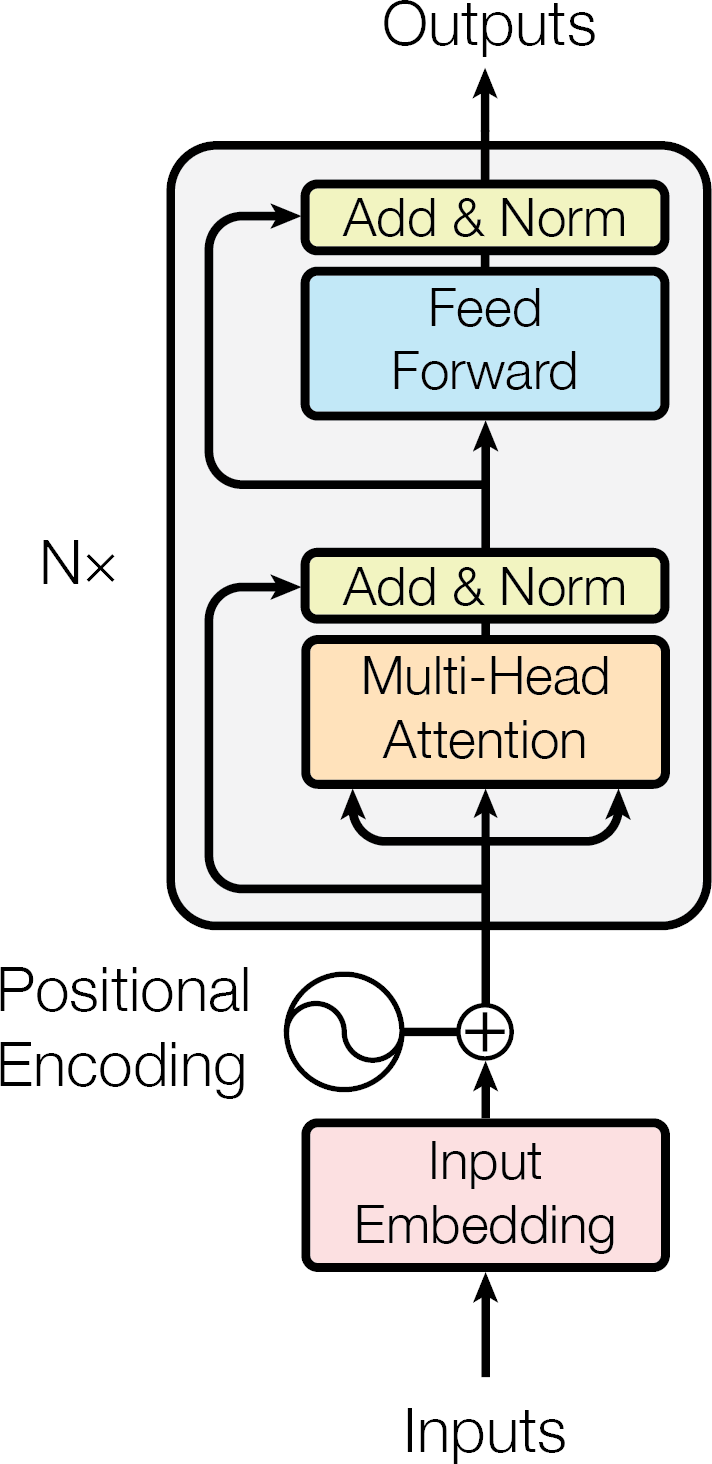
\includegraphics[width=\textwidth]{images/Transformer/TF_Encoder.png}

      \caption{Overview of the Transformer Encoder.}
      \label{fig:encoder}
    \end{subfigure}
    \hspace{0.2\textwidth}
    \begin{subfigure}{0.2\textwidth}
        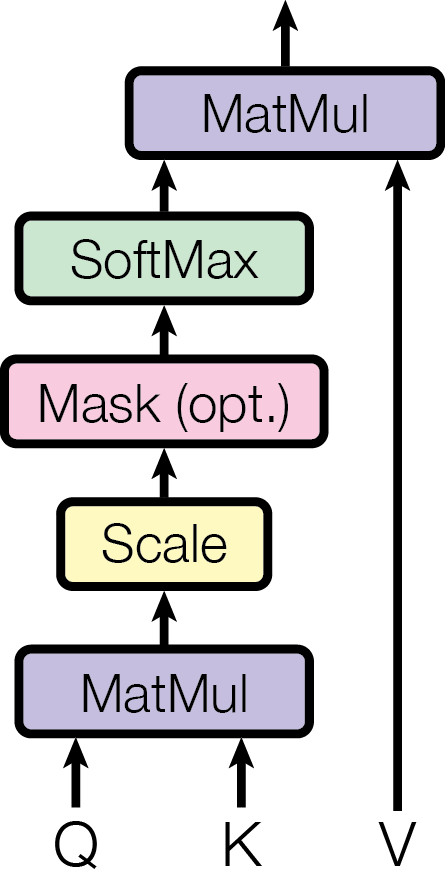
\includegraphics[width=\textwidth]{images/Transformer//AttentionHead.png}
        \caption{Attention Mechanism.}
      \label{fig:selfattention}
    \end{subfigure}
    \caption{Transformer Encoder Architecture. Figures taken from \cite{vaswani2017attention}.}
    \label{fig:transformer}
  \end{figure}

The idea of attention can be explained as follows: given a set of inputs, the model learns to assign a weight to each input based on its relevance to the 
task at hand.
This weighted sum of inputs is then used as a representation of the input sequence. One of the most successful architectures for attention based sequence models is the Transformer developed by Vaswani \etAl \cite{vaswani2017attention}. In the paper, the transformer 
consists of an encoder and a decoder.

The Transformer architecture consists of an encoder and a decoder, each containing multiple layers of self-attention and feedforward neural networks. 
In the self-attention layer, each input token is transformed into a query $Q$, key $K$, and value $V$ vector. 
The vectors $Q$, $K$ and $V$ are computed using a position wise feed forward network with ReLU activation:
\begin{equation}
    QKV = \text{ReLU}(x \ W_1 + b1)W_2 + b_2,
\end{equation}
where the same weights $W_n$ and biases $b_n$ are used for every input $x$ of the sequence. This is expected to be an advantage following the BIC argument from Section \ref{COD}. 
These vectors are used to compute the attention weights between each pair of input tokens.
The resulting weighted sum of value vectors is used as the output of the self-attention layer.
The attention weights are computed as follows:
\begin{equation}
\text{Attention}(Q, K, V) = \text{softmax}\left(\frac{QK^T}{\sqrt{d_k}}\right)V,
\end{equation}
where $d_k$ is the dimensionality of the key vectors.
The softmax function normalizes the dot product of $Q$ and $K$, which represents the similarity between the query and key vectors.
The attention weights represent the importance of each value vector in the weighted sum. They can then be input to an MLP to compute the result.
 
Note with this setup, the model has no way to encode the relative position of the tokens, which is why a positional encoding is added along the sequence dimension, 
using sine and cosine functions, to break the symmetry.

In this thesis, we will use transformer encoder to model our neural networks. They only consists of self attention and the output MLP, as depicted in Figure \ref{fig:transformer}. 
We will not describe the whole transformer architecture, 
as in this thesis we only make use of the encoder architecture.

One advantage of the Transformer architecture is that it does not suffer from the problem of vanishing or exploding gradients.
This is because the self-attention mechanism allows the model to directly access any input token, without the need for recurrent connections. Self attention type 
architectures have been shown to outperform recurrent networks on a number of sequence based tasks. For example they are used in the GPT-3 architecture, which has 
shown impressive results in natural language prediction \cite{brown2020language}. While they were developed for natural language tasks, they have 
shown promising results in a multitude of areas, including image generation, image classification, \ac{il} and \ac{rl}.